\documentclass[a4paper, 12pt]{article}

\usepackage{custom}
\usepackage{graphicx}
\usepackage{float}

%--------------------VARIABILI--------------------
\def\lastversion{v1.0}
\def\title{Manuale Utente}
\def\date{04 Giugno 2025}
%------------------------------------------------

\begin{document}

\primapagina


\begin{registromodifiche}
    \hline
    \lastversion & 04 Giugno 2025 &  & Enrico Bianchi & Release \\
    \hline
        v0.1 & 04 Giugno 2025 & Francesco Savio & Guirong Lan & Realizzazione manuale utente \\
    \hline
\end{registromodifiche}

\tableofcontents

\newpage

\section{Introduzione}
\label{sec:introduzione}

\subsection{Scopo del documento}
Il presente documento è dedicato a fornire una panoramica delle caratteristiche di \textit{Artificial QI}. Attraverso questa guida l’utente potrà gestire un dataset.
Il manuale contiene istruzioni dettagliate per accompagnare l’utente nell’utilizzo di \textit{Artificial QI}, illustrando passo dopo passo le opzioni disponibili.

\subsection{Riferimenti}

\subsubsection{Normativi}

\begin{enumerate}
    \item Capitolato C1 - Artificial QI: \href{https://www.math.unipd.it/~tullio/IS-1/2024/Progetto/C1.pdf}{ArtificialQI}

    \item Norme di progetto v2.0.
\end{enumerate}

\subsubsection{Informativi}

\begin{enumerate}
    \item Analisi dei requisiti 2.0.
    \item Specifica tecnica v1.0.
    \item Glossario v1.0.
\end{enumerate}
Tutti i documenti prodotti dal gruppo sono disponibili al seguente link \href{https://alt-f4-eng.github.io/Documentazione/}{https://alt-f4-eng.github.io/Documentazione/}

\section{Requisiti}
\label{sec:requisiti}

\subsection{Requisiti hardware}
\begin{itemize}
  \item \textbf{Processore}: almeno un dual-core a 1,2 GHz
  \item \textbf{Memoria RAM}:
    \begin{itemize}
      \item \emph{Minimo}: 2 GB
      \item \emph{Consigliato}: 4 GB o più (per prestazioni ottimali)
    \end{itemize}
  \item \textbf{Spazio su disco}: almeno 5 GB di spazio libero
  \item \textbf{Connessione Internet}: necessaria per accedere ai servizi e APIs
\end{itemize}

\subsection{Requisiti software}

Per eseguire correttamente l’applicazione, è necessario avere Docker installato. I requisiti specifici sono:\\

\textbf{Windows - MacOS - Linux}
\begin{enumerate}
    \item \textit{Docker Desktop}
    \begin{itemize}
        \item Docker Desktop fornisce Docker Engine, Docker Compose e tutte le librerie necessarie per l’esecuzione dei container.
        \item Ulteriori dettagli sono disponibili qui: \href{https://www.docker.com/products/docker-desktop/}{https://www.docker.com/products/docker-desktop/}
    \end{itemize}
    
\end{enumerate}


\subsection{Browser supportati}

Di seguito sono elencati i browser in cui l’applicazione è accessibile:

\begin{table}[H]
\centering
\begin{tabular}{ll}
\hline
    \textbf{Browser} & \textbf{Versione} \\
    \hline
    Google Chrome     & 124 e successive \\
    \hline
    Mozilla Firefox   & 115 e successive \\
    \hline
    Safari            & 16 e successive  \\
    \hline
    Microsoft Edge    & 124 e successive \\
    \hline
\end{tabular}
\caption{Tabella dei browser supportati}
\label{tab:browser_supportati}
\end{table}



\section{Installazione}
\label{sec:installazione}

Per installare l'applicazione è necessario scaricare il codice sorgente dal \glossario{repository} in una cartella dedicata.\\
Il \glossario{repository} è disponibile a questo link - \href{https://github.com/ALT-F4-eng/ArtificialQI}{https://github.com/ALT-F4-eng/ArtificialQI}
Per scaricare il codice sorgente vi sono due modalità principali:
\begin{itemize}
    \item Scaricare il repository in formato zip e decomprimerlo in una cartella dedicata
    \item Clonare il repository tramite il seguente comando:\\
     git clone https://github.com/ALT-F4-eng/ArtificialQI.git
\end{itemize}

\section{Avvio}
\label{sec:avvio}

L’applicazione può essere avviata, dopo essersi posizionati con il terminale nella cartella del progetto, tramite i seguenti comandi:
\begin{itemize}
    \item docker compose build
    \item docker-compose up
\end{itemize}
Una volta avviata l’applicazione, è possibile accedervi tramite il browser all’indirizzo http://localhost:4200.

\section{Utilizzo}
\label{sec:utilizzo}

La sezione seguente presenta le funzionalità del sistema.

\subsection{Sezione Home}
\label{subsec:sezione_home}

La sezione Home è una pagina interamente descrittiva che presenta le funzionalità generali dell'applicazione.

\subsection{Sezione Dataset}
\label{subsec:sezione_dataset}

\begin{figure}[H]
    \centering
    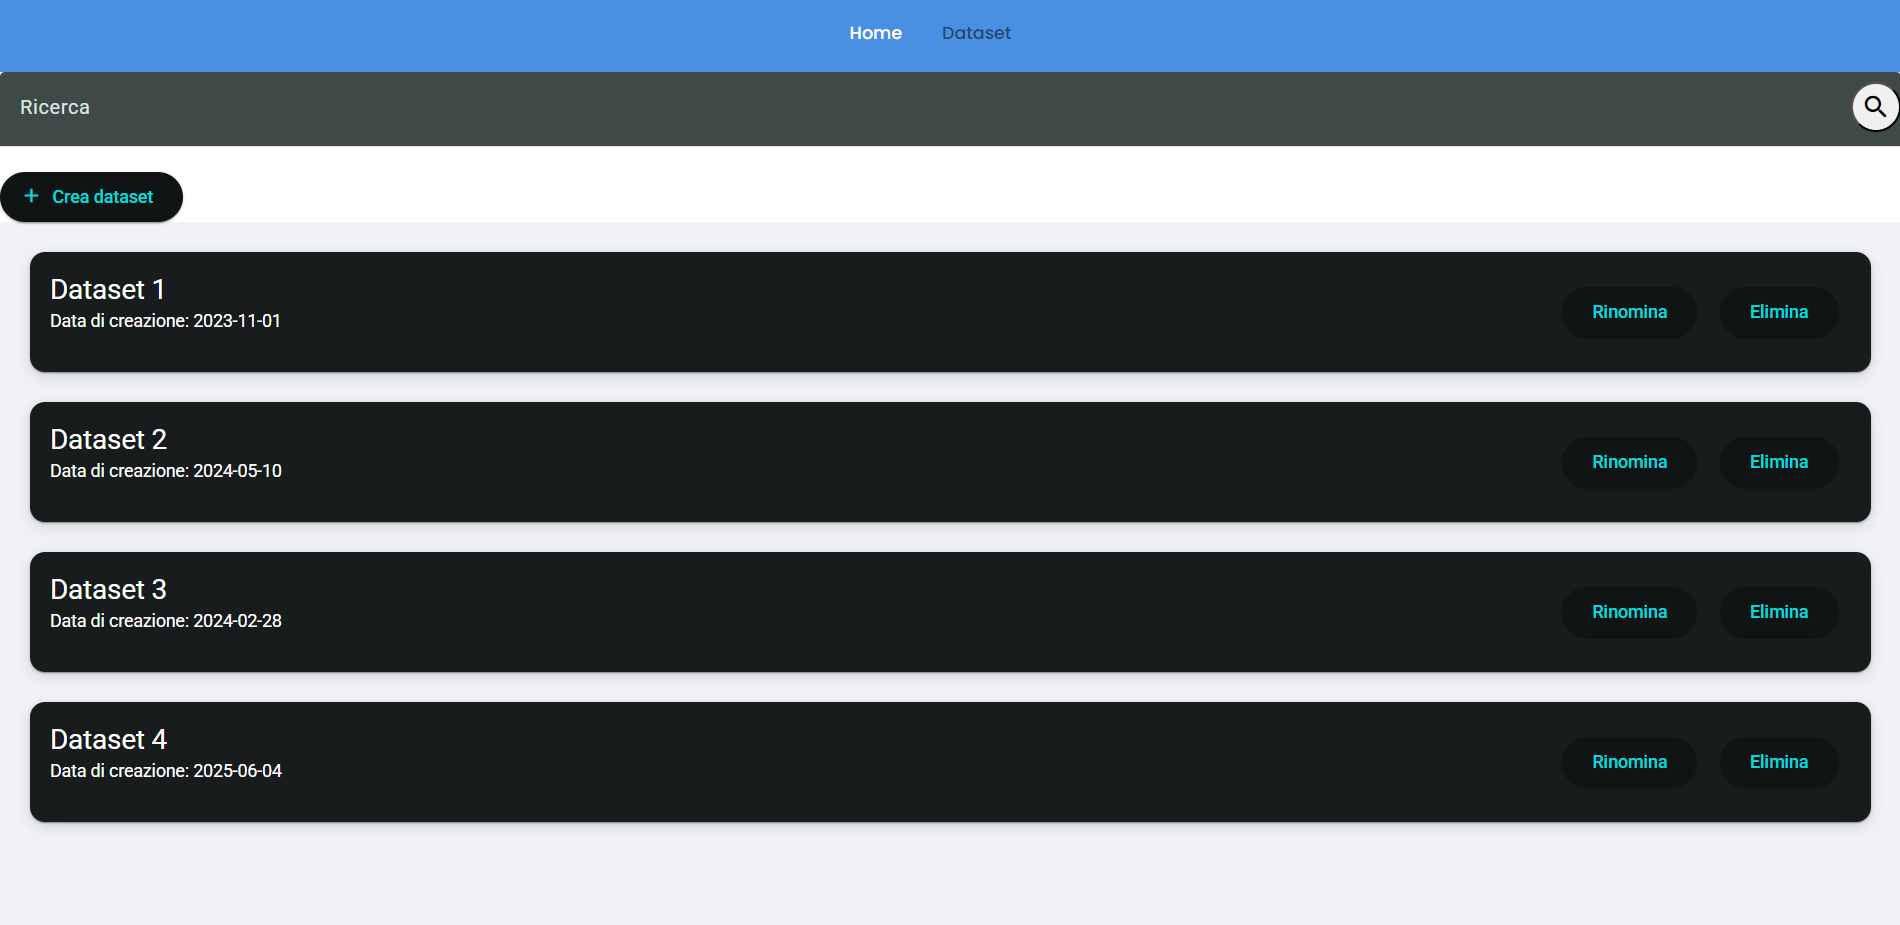
\includegraphics[scale=0.35]{Sezioni/Requisiti/immagini/dataset.png}
\end{figure}

La sezione Dataset è composta da tre elementi principali:
\begin{itemize}
    \item Barra di ricerca - Attraverso la barra di ricerca posizionata nella parte superiore della pagina è possibile filtrare la lista dei dataset per nome.
    \item Bottone crea dataset - Attraverso il bottone crea dataset è possibile aggiungere un nuovo dataset alla lista attraverso un form pop-up che richiederà l'inserimento di un nome.
    \begin{figure}[H]
    \centering
    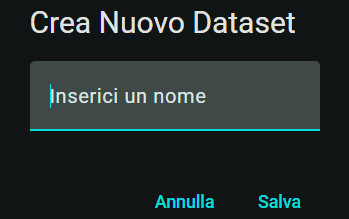
\includegraphics[scale=0.6]{Sezioni/Requisiti/immagini/nuovo_dataset.png}
    \end{figure}
    \item Lista dataset - Qui saranno visualizzati tutti i dataset salvati con i relativi bottoni che consentono di rinominare un dataset oppure eliminarlo con una richiesta pop-up.
    \begin{figure}[H]
    \centering
    
    \begin{minipage}[b]{0.48\textwidth}
        \centering
        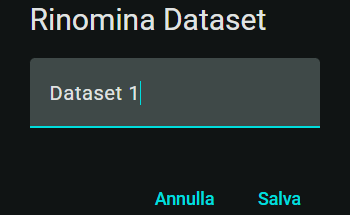
\includegraphics[scale=0.5]{Sezioni/Requisiti/immagini/rinomina_dataset.png}
    \end{minipage}
    \hfill
    \begin{minipage}[b]{0.48\textwidth}
        \centering
        
\includegraphics[scale=0.5]{Sezioni/Requisiti/immagini/elimina_dataset.png}
    \end{minipage}
    \end{figure}
\end{itemize}
Infine il sistema notificherà l'utente con l'esito di ogni operazione fornendo una conferma o un errore in modo dinamico.
\begin{figure}[H]
    \centering
    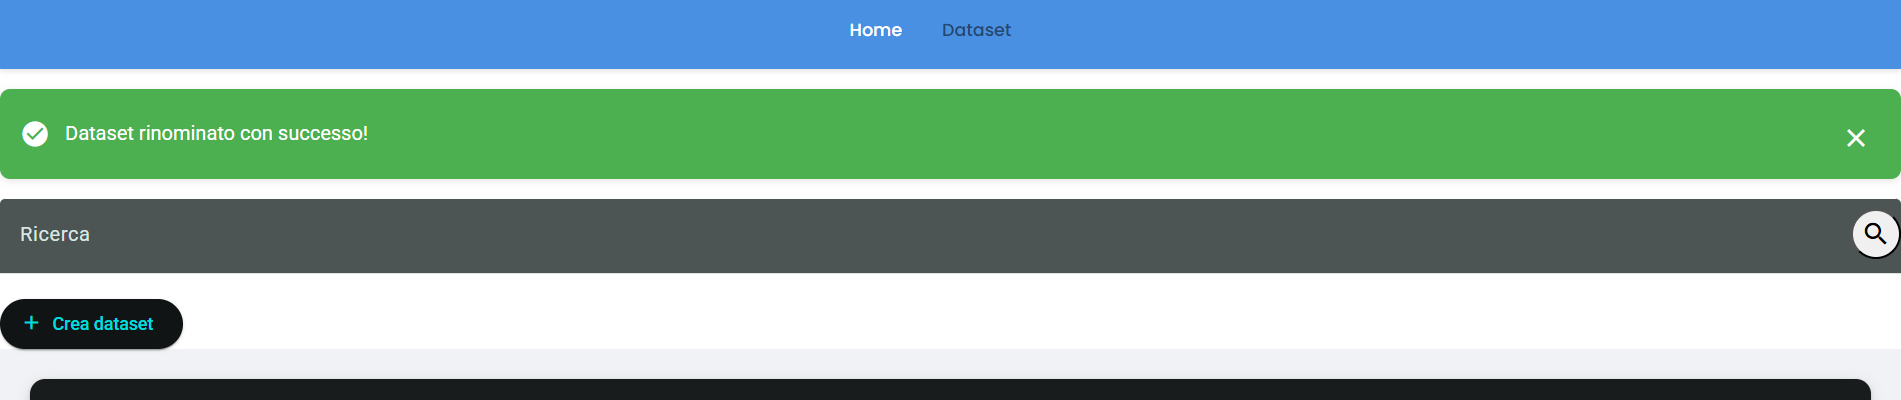
\includegraphics[scale=0.35]{Sezioni/Requisiti/immagini/notificav.png}
\end{figure}
\begin{figure}[H]
    \centering
    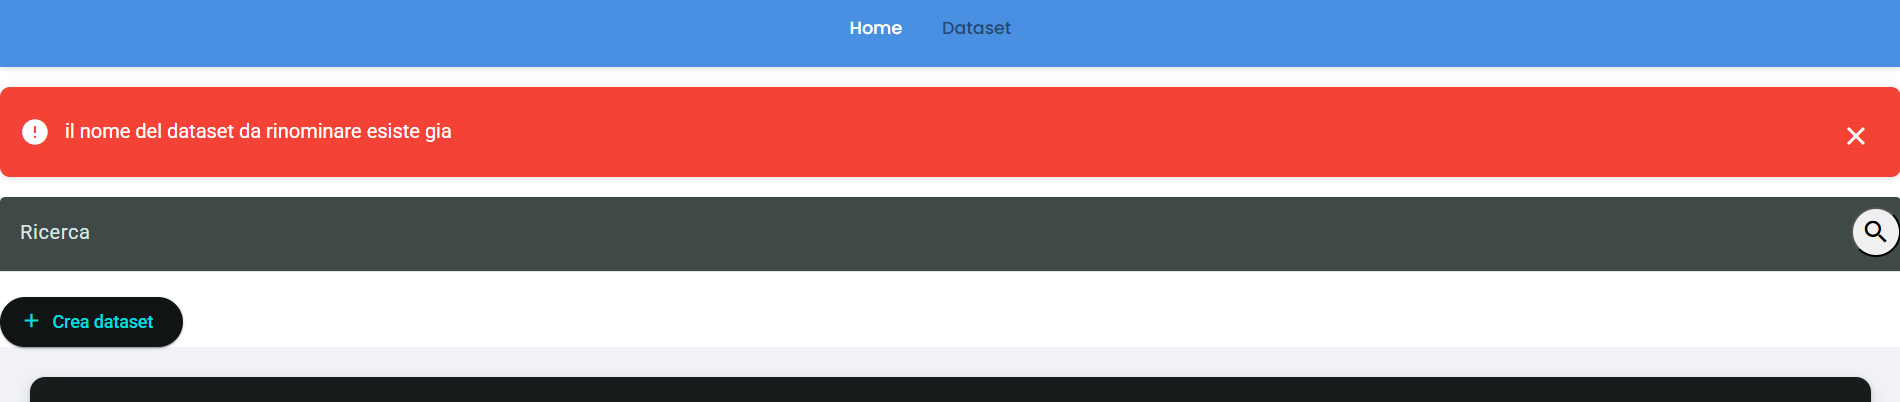
\includegraphics[scale=0.35]{Sezioni/Requisiti/immagini/notificax.png}
\end{figure}

%\section{Istruzioni all'utilizzo}
\label{sec:istruzioni_utilizzo}

\input{Sezioni/IstruzioniUtilizzo/Sottosezioni/.tex}

\input{Sezioni/IstruzioniUtilizzo/Sottosezioni/.tex}

\input{Sezioni/IstruzioniUtilizzo/Sottosezioni/.tex}

\end{document}